% This is auto-generated file: do not edit!
% Exported from microMathematics Plus, version 2.17.2


Este exemplo demonstra desenhos 3D para
três funções diferentes de duas
variáveis.

Primeiro, definimos intervalos para os
argumentos x e y. O intervalo para o
eixo x depende do número de pontos
juntamente com os valores mínimo e
máximo do eixo x, x1 e x2:
\begin{center}\begin{tabular}{ccc}
  $N := 300$ &
  $x1 := -2$ &
  $x2 := 2$ \cr
\end{tabular}\end{center}
\begin{center}\begin{tabular}{c}
  $x := \left[ x1,\, x1 +  \left| x2 - x1 \right|  / N \,..\, x2 \right]$
\end{tabular}\end{center}

O intervalo para o eixo y é definido
analogamente:
\begin{center}\begin{tabular}{ccc}
  $M := 300$ &
  $y1 := -3$ &
  $y2 := 3$ \cr
\end{tabular}\end{center}
\begin{center}\begin{tabular}{c}
  $y := \left[ y1,\, y1 +  \left| y2 - y1 \right|  / M \,..\, y2 \right]$
\end{tabular}\end{center}

Por exemplo, deixe-nos desenhar uma
função trigonométrica que é um produto
de seno e cosseno:
\begin{center}\begin{tabular}{c}
  $F(x,y) := sin \left( 3 \cdot {x}^{2}\right)  \cdot cos \left( {y}^{2}\right) $
\end{tabular}\end{center}

Para criar uma visualização 3D, toque
no botão ''Novo elemento'' da barra de
ações ou pelo botão ''Adicionar desenho
3D'' da barra de ferramentas:
\begin{center}\begin{tabular}{c} 
\includegraphics[resolution=320]{graphics/three_d_plot_fig1.png} \end{tabular}\end{center}

Coloque o nome da função F(x,y) no
campo central-inferior:
\begin{center}\begin{tabular}{c} 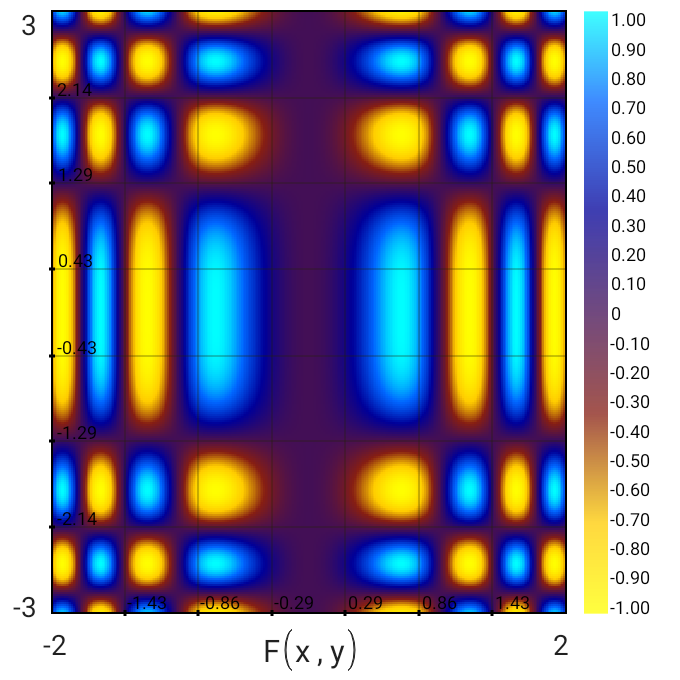
\includegraphics[resolution=320]{graphics/three_d_plot_fig2.png} \end{tabular}\end{center}

Os limites do desenho, tamanho do
traçado e aparência, rótulos e grade
podem ser ajustados por analogia com a
função de desenho usando a janela de
configurações do desenho (veja o
exemplo ''Desenhar Função'' da gaveta de
aplicações do app para mais detalhes).
Para abrir esta janela, toque na área
de desenho até que o botão flutuante
''Propriedades do objeto'' apareça, e
então toque neste botão.

Adicionalmente, você pode alterar o
número de rótulos no eixo z e escolher
a paleta de cores na janela
''Configurações do Mapa de Cores''. Esta
janela aparece tocando demoradamente
na barra do eixo z à direita da área
principal do gráfico.
\begin{center}\begin{tabular}{c}
  $R(x,y) := sin \left( 5 \cdot {x}^{2} \cdot \left( y - x \right)\right) $
\end{tabular}\end{center}
\begin{center}\begin{tabular}{c} 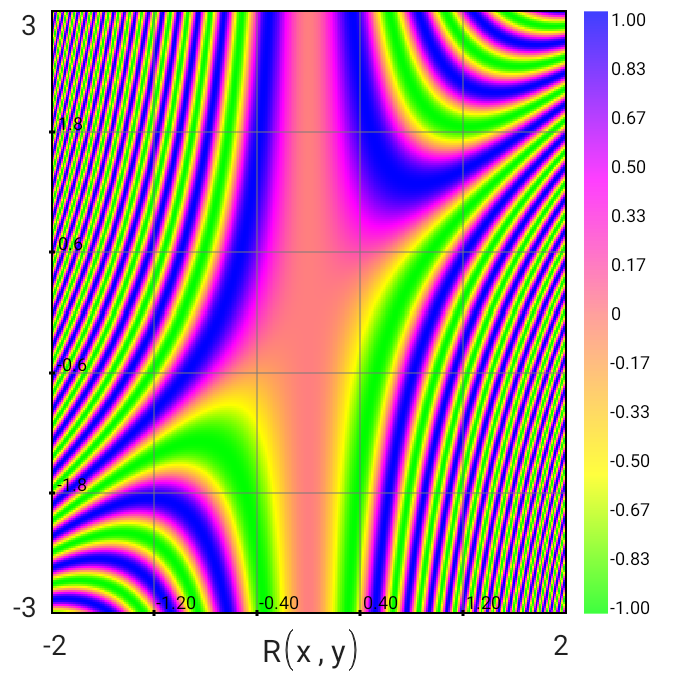
\includegraphics[resolution=320]{graphics/three_d_plot_fig3.png} \end{tabular}\end{center}

Uma função de dois argumentos também
pode ser desenhada como uma superfície
no espaço 3D. Este modo pode ser
ativado na janela de ''Configurações de
Desenho'' que aparece se você tocar no
botão flutuante ''Propridades do
objeto'' após tocar demoradamente na
área de desenho. Deixe-nos desenhar a
seguinte função, usando conjuntos para
poder diminuir o tempo de cálculo:
\begin{center}\begin{tabular}{cccc}
  $N := 100$ &
  $n := \left[ 0,\, 1 \,..\, N \right]$ &
  $x1 := -15$ &
  $x2 := 15$ \cr
\end{tabular}\end{center}
\begin{center}\begin{tabular}{cccc}
  $M := 100$ &
  $m := \left[ 0,\, 1 \,..\, M \right]$ &
  $y1 := -15$ &
  $y2 := 15$ \cr
\end{tabular}\end{center}
\begin{center}\begin{tabular}{c}
  $x[n] := {\left( x1 +  \left( x2 - x1\right)  \cdot n / N \right)}^{2}$
\end{tabular}\end{center}
\begin{center}\begin{tabular}{c}
  $y[m] := {\left( y1 +  \left( y2 - y1\right)  \cdot m / M \right)}^{2}$
\end{tabular}\end{center}
\begin{center}\begin{tabular}{c}
  $r[n,m] := 0.04 \cdot x_{n}  + 0.02 \cdot y_{m} $
\end{tabular}\end{center}
\begin{center}\begin{tabular}{c}
  $t[n,m] := \left( x_{n}  + 0.05 \cdot y_{m}  \right) \cdot exp \left( 1 - r_{n,\, m} \right) $
\end{tabular}\end{center}
\begin{center}\begin{tabular}{c}
  $F[n,m] := \frac{sin \left( x_{n}  + 0.1 \cdot y_{m} \right) }{0.15 + r_{n,\, m} } + \frac{t_{n,\, m} }{10}$
\end{tabular}\end{center}
\begin{center}\begin{tabular}{c} 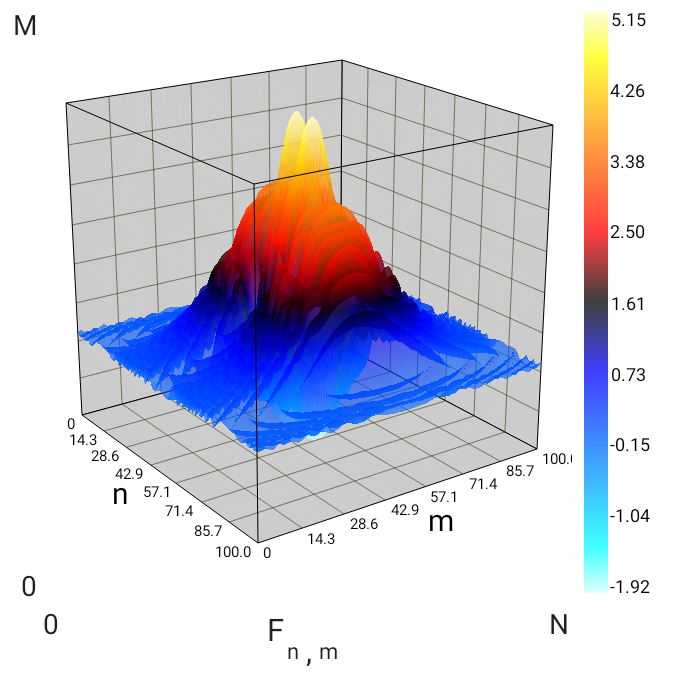
\includegraphics[resolution=320]{graphics/three_d_plot_fig4.png} \end{tabular}\end{center}

Para o desenho de superfícies, existem
configurações adicionais mostradas na
janela de ''Configurações de Desenho''.
Você pode escolher se deseja que as
linhas da malha devem ser mostradas.
Selecione a opacidade para a cor da
malha, defina os ângulo de rotação e a
elevação da caixa de desenho. Por
exemplo, a superfície desenhada
anteriormente com outros ângulos de
rotação e elevação se parece com: 
\begin{center}\begin{tabular}{c} 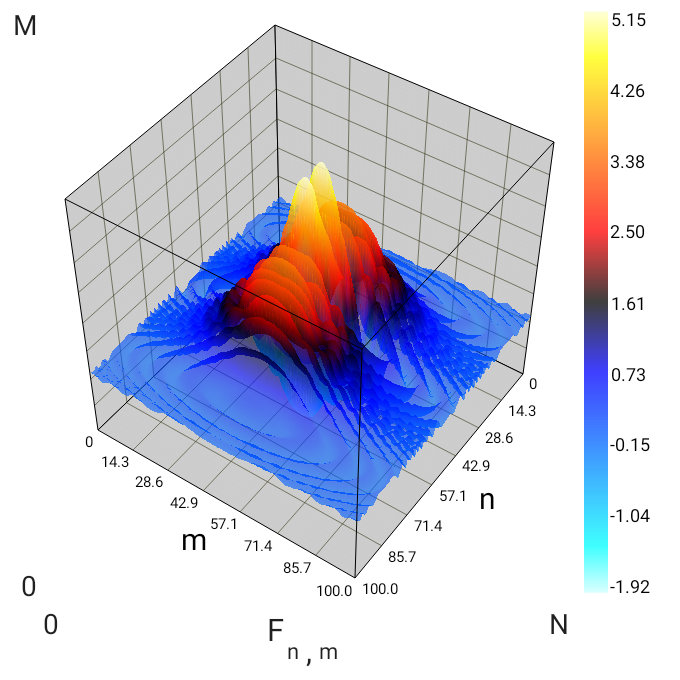
\includegraphics[resolution=320]{graphics/three_d_plot_fig5.png} \end{tabular}\end{center}